% <- percent signs are used to comment
\documentclass[12pt]{article}

%%%%%% PACKAGES - this part loads additional material for LaTeX %%%%%%%%%
% Nearly anything you want can be done in LaTeX if you load the right package 
% (search ctan.org or google it if you are looking for something).  We will load
% here a few that we need for this document or that we expect you to need later.

% The next 3 lines are needed to fix shortcomings of TeX that only make sense given its 40-year history ...
% Simple keep and ignore.
\usepackage[utf8]{inputenc}
\usepackage[T1]{fontenc}
\usepackage{lmodern}
\usepackage{amsmath}
\usepackage{changepage}
\usepackage{lipsum}
\usepackage{tikz}


% Custom margins (and paper sizes etc.) because LaTeX else wastes much space
\usepackage[margin=1in]{geometry}

% The following packages are created by the American Mathematical Society (AMS)
% and provide lots of tools for special fonts, symbols, theorems, and proof
\usepackage{amsmath,amsfonts,amssymb,amsthm}
% mathtools contains many detail improvements over ams and core tex
\usepackage{mathtools}

% graphicx is required for images
\usepackage{graphicx}

% enumitem used for customizing enumerations
\usepackage[shortlabels]{enumitem}

% tikz is the package used for drawing, in particular for drawing trees. You may also find simplified packages like tikz-qtree and forest useful
\usepackage{tikz}

% hyperref allows links, urls, and many other PDF tricks.  We load it here
%          in such a way that the PDF file has info about it
\usepackage[%
	pdftitle={CS240 Assignment 0},%
	hidelinks,%
]{hyperref}


%%%%%% COMMANDS - here you can define your own LaTeX-commands %%%%%%%%%

%%%%%% End of Preamble %%%%%%%%%%%%%

\begin{document}

\begin{center}
{\Large\textbf{CS240, Spring 2022}}\\
\vspace{2mm}
{\Large\textbf{Assignment 4: Question 2}}\\
\vspace{3mm}
\end{center}
\begin{adjustwidth}{0em}{0pt}
\textbf{Q2a)} 
\begin{figure}[tbhp]
	\begin{center}
		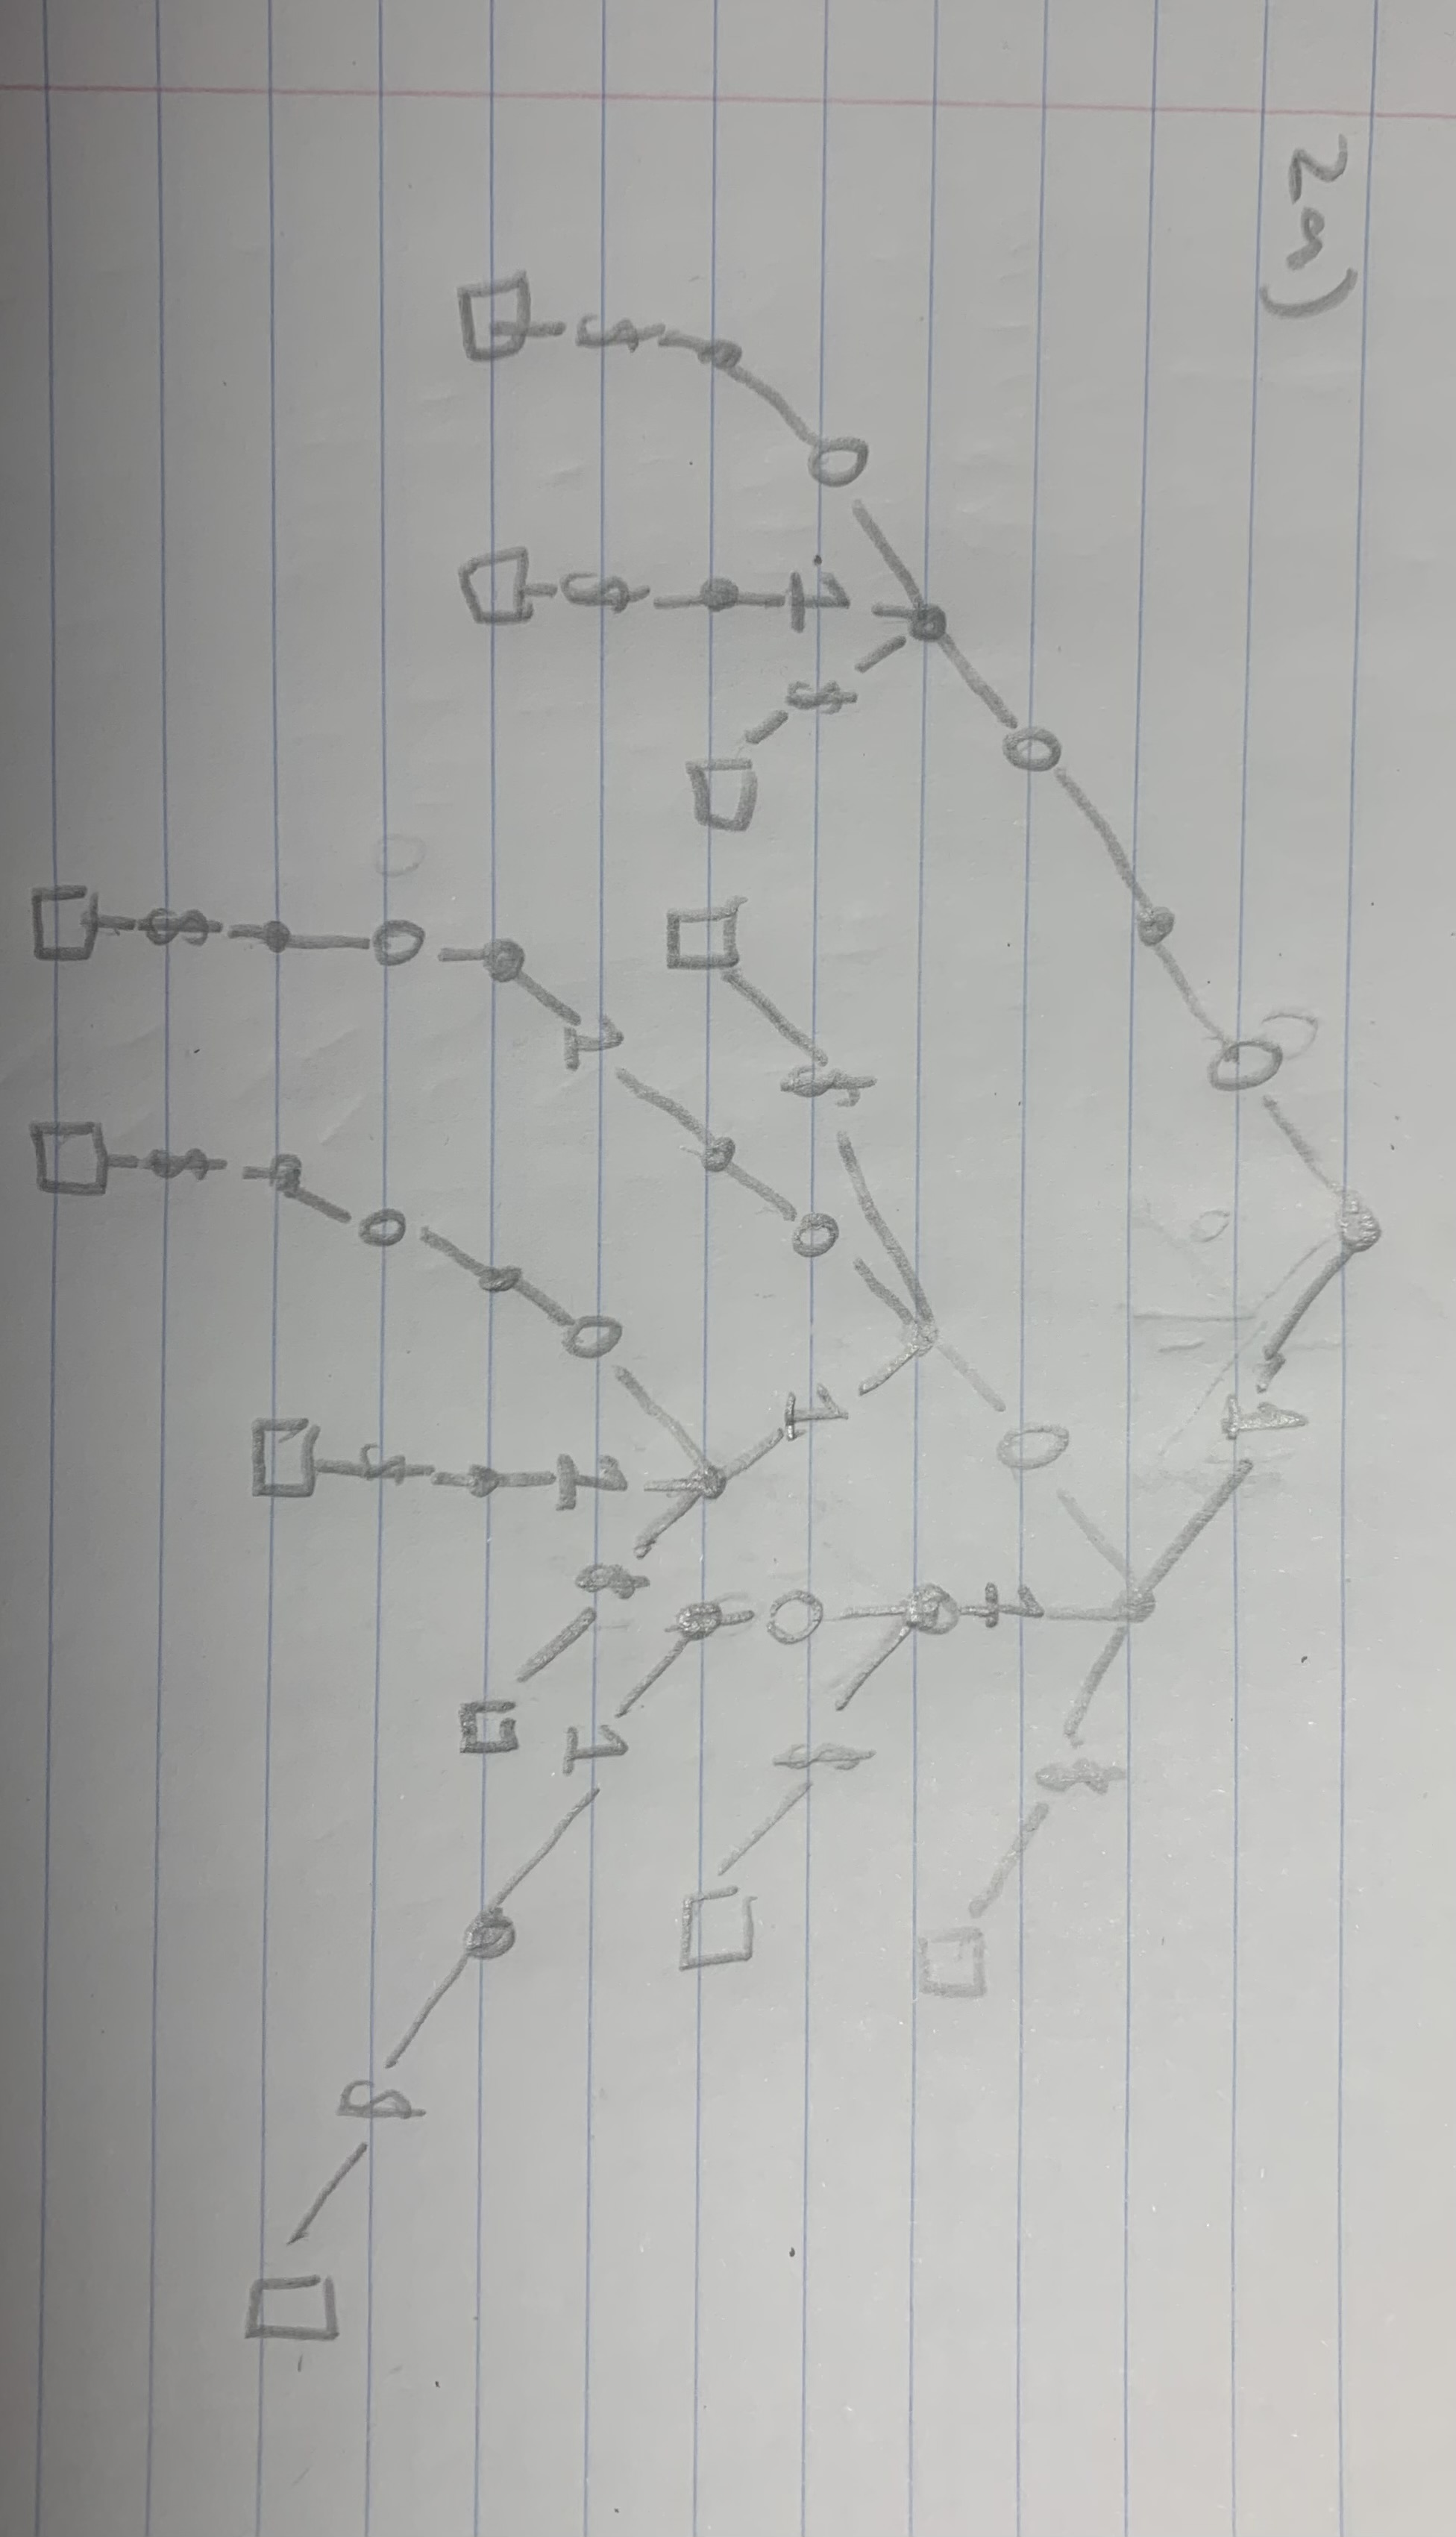
\includegraphics[width=0.6\textwidth, angle=90]{2a.jpg}
	\end{center}
\end{figure}
\end{adjustwidth} 
\newpage
\begin{adjustwidth}{0em}{0pt}
\textbf{Q2b)}
\begin{figure}[tbhp]
	\begin{center}
		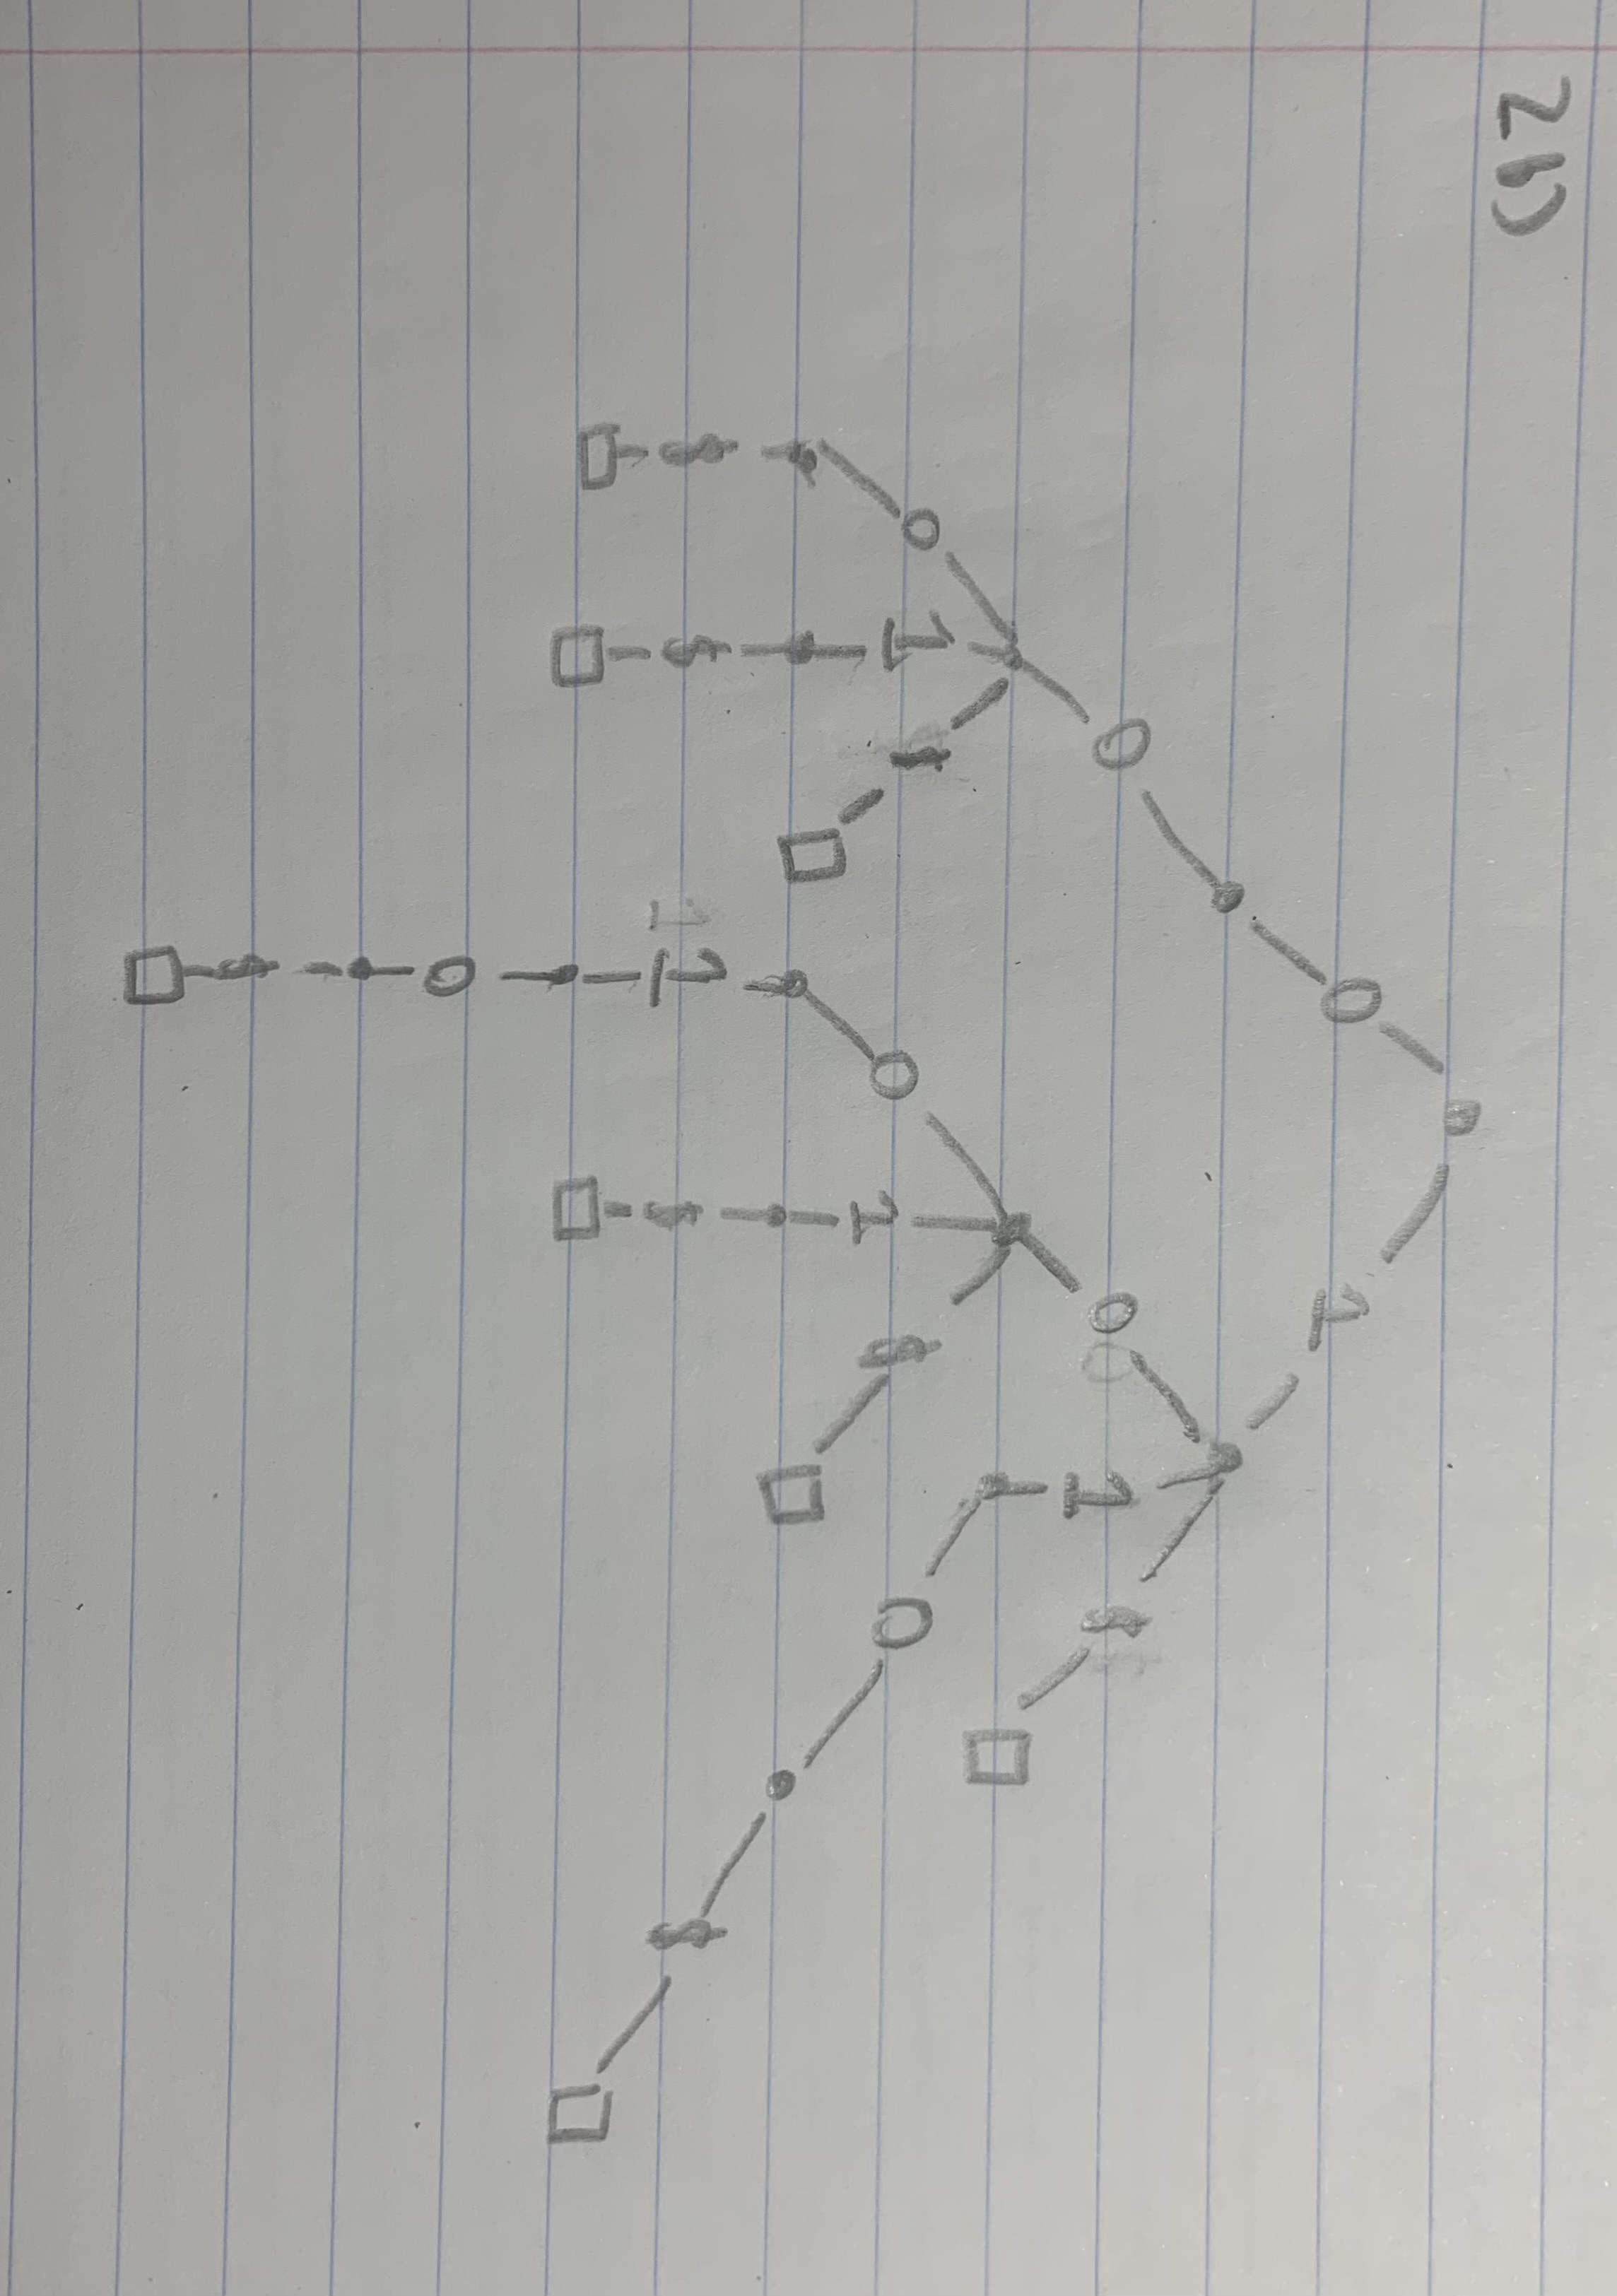
\includegraphics[width=0.7\textwidth, angle=90]{2b.jpg}
	\end{center}
\end{figure}
\end{adjustwidth} 
\newpage
\begin{adjustwidth}{0em}{0pt}
\textbf{Q2c)} 
\begin{figure}[tbhp]
	\begin{center}
		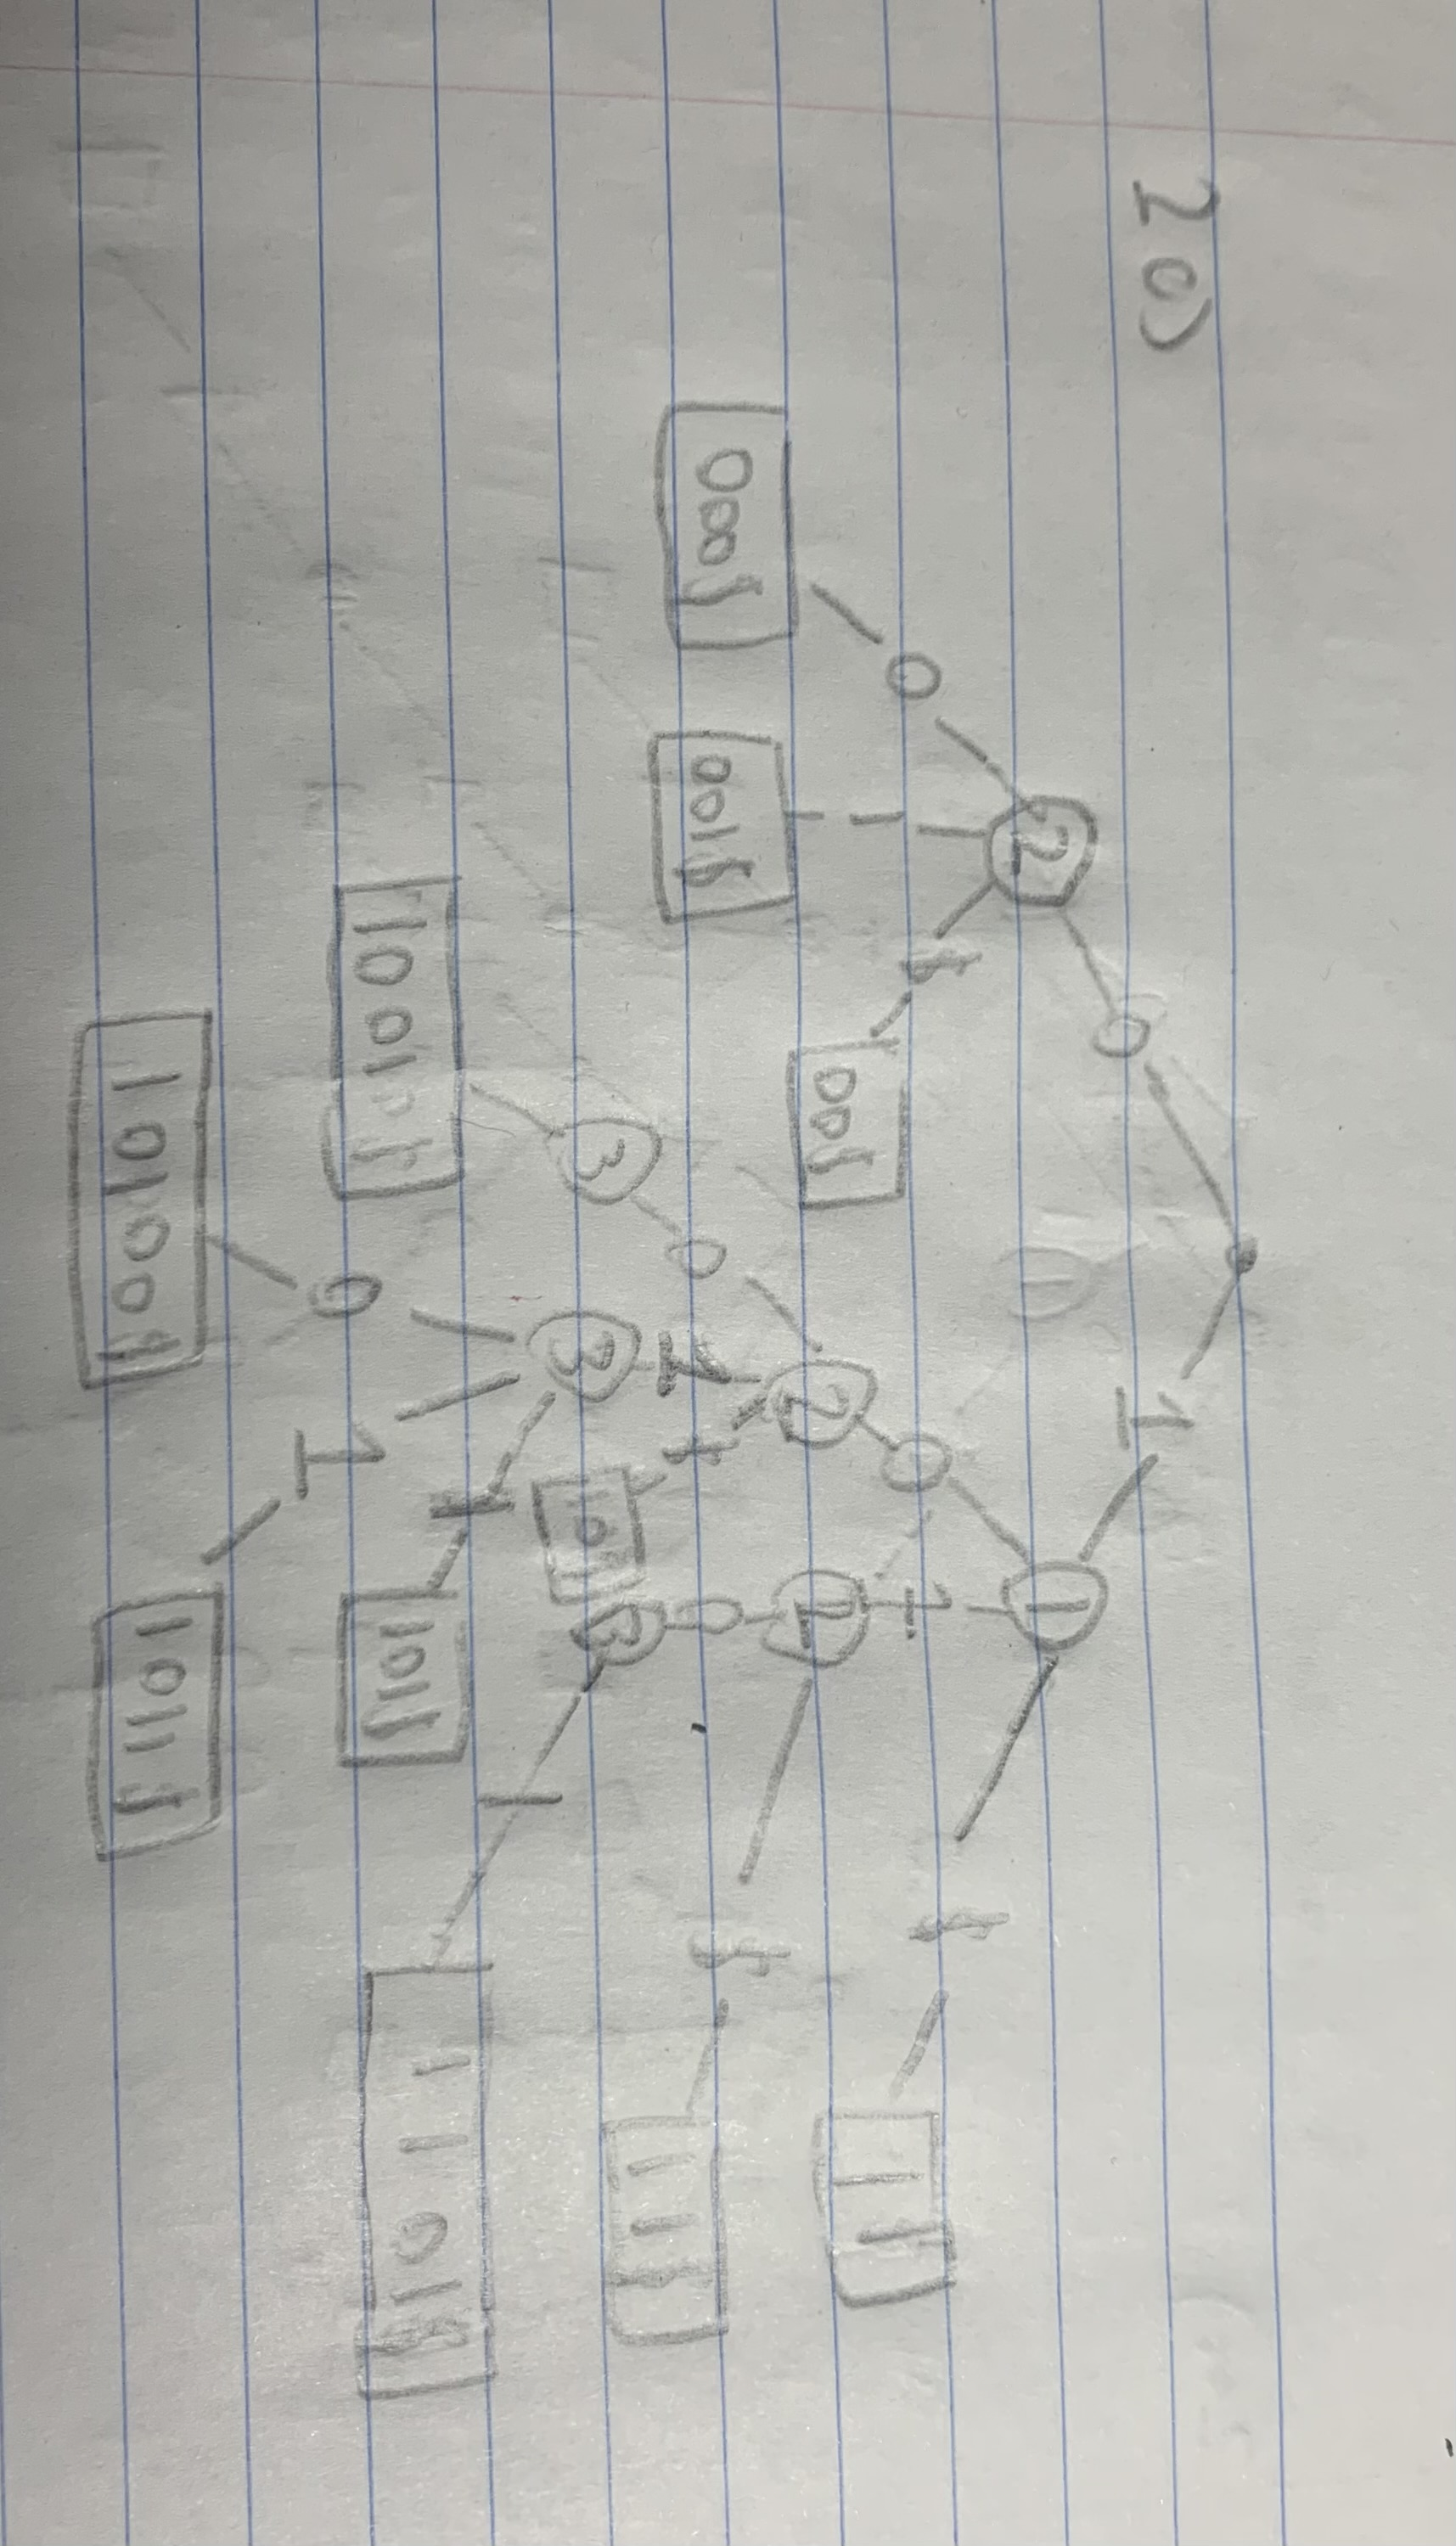
\includegraphics[width=0.6\textwidth, angle=90]{2c.jpg}
	\end{center}
\end{figure}
\end{adjustwidth} 
\newpage
\begin{adjustwidth}{0em}{0pt}
\textbf{Q2d)}
\begin{figure}[tbhp]
	\begin{center}
		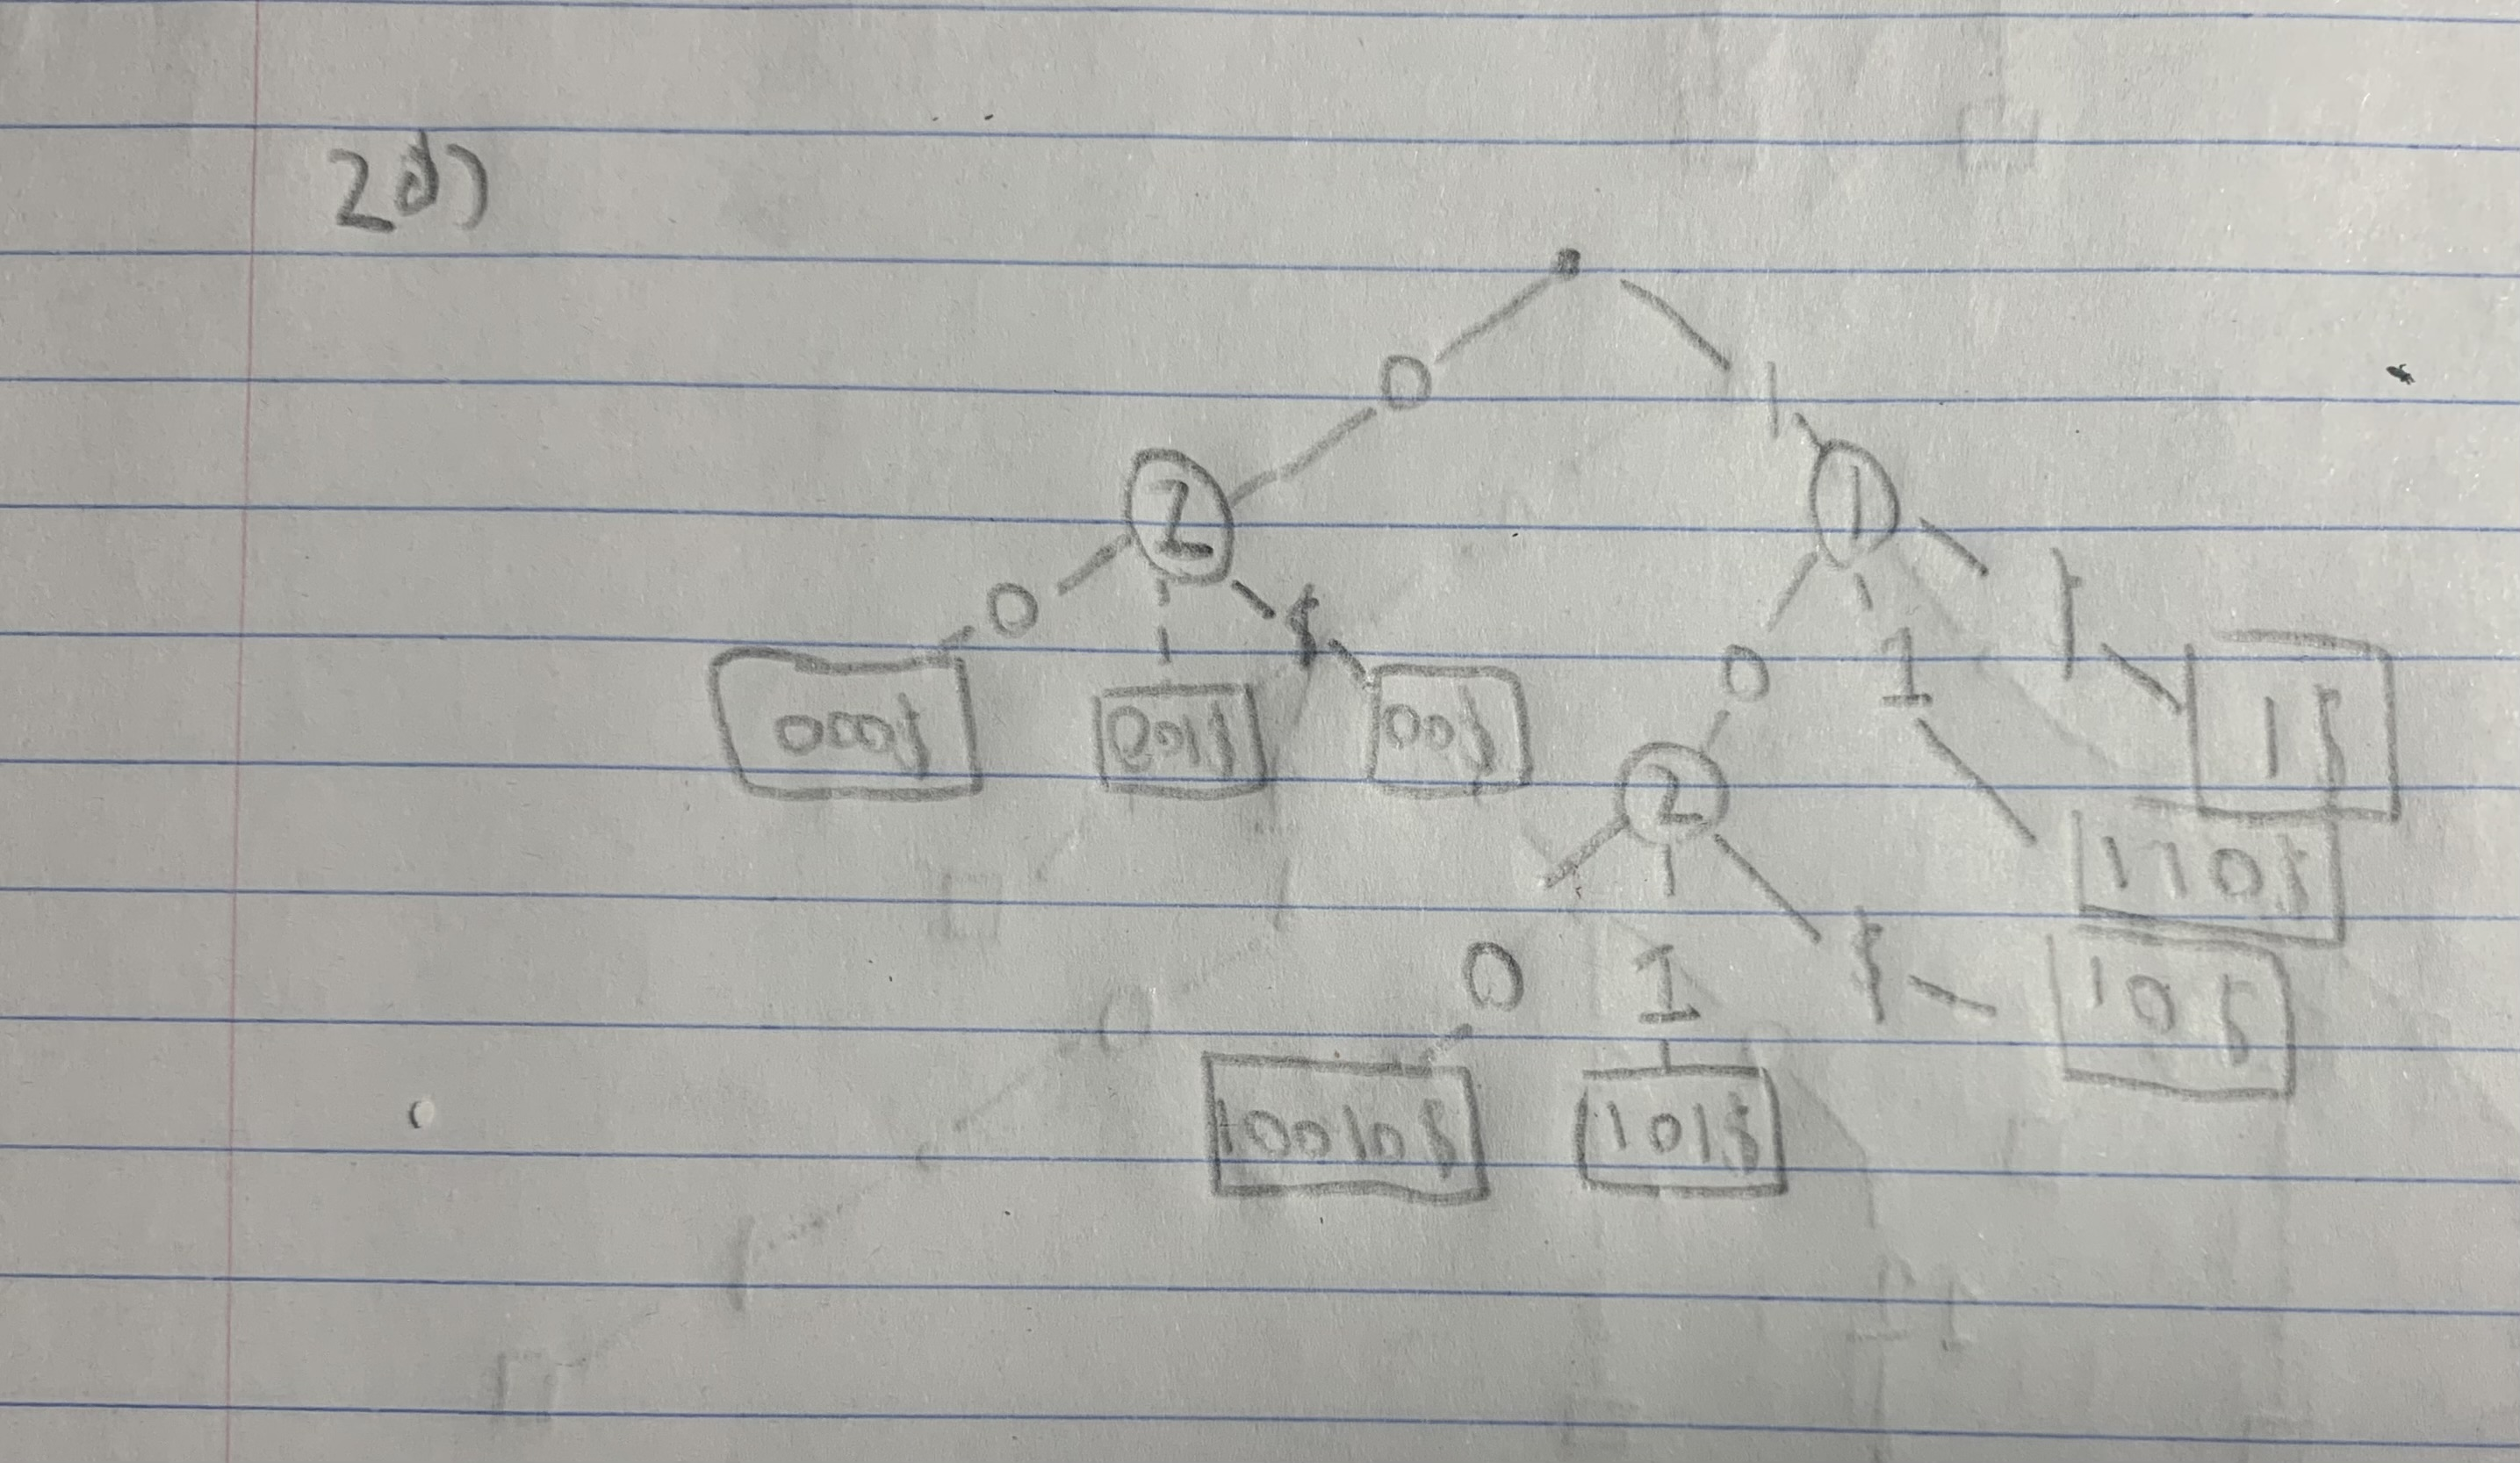
\includegraphics[width=1\textwidth, angle=0]{2d.jpg}
	\end{center}
\end{figure}
\end{adjustwidth} 
\newpage
\begin{adjustwidth}{0em}{0pt}
\textbf{Q2e)} Find the exact height of the trie with keys that are binary representations of numbers $0, 1, 2, 3, 4, ..., 2^{k-1}$ without leading 0s, and inserted into the trie in increasing order. That is, insert 0\$, 1\$, 10\$, 11\$, 100\$, etc. Justify your answer. \\\\
In order to generate an $d$ digit number with no leading zeros for all $n > 1$ the first value needs to be 1 and for each of the $n-1$ remaining positions we can have either 1 or zero. Thus the total count of d digit numbers with no zeros is given by (where $d > 1$):
\[ = 2^{d-1} \]
Thus we will at level $i$ on our trie we have:
\[ = 2^{i-1} (\text{total combinations of i digit numbers})) \]
We can get an equation for an inserted value $n$ where it is proportional to its height $h$ in the trie:
\[ n = \sum^h_{i=2}(2^{i-1}) \]
However since note that this doesn't account for the last level in our trie which is just nodes of \$. Thus accounting for that we get:
\[ n = \sum^{h-1}_{i=2}(2^{i-1}) \]
Since we know the last node we insert is $2^{k-1}$, thus since the last node will be the largest we can use it to gage the height of the trie. Thus we get:
\begin{align*}  
    \begin{aligned}
       2^{k} -1 &= \sum^{h-1}_{i=2}(2^{i-1}) \\
       2^{k} -1  &= \sum^{h-1}_{i=0}(2^{i-1}) - 1 - \frac{1}{2}\\
       2^{k} + \frac{1}{2}  &= \sum^{h-1}_{i=0}(2^{i-1})\\
       2^{k} + \frac{1}{2}  &=\frac{1}{2}\sum^{h-1}_{i=0}(2^{i})\\
       2^{k+1} + 1 &= \sum^{h-1}_{i=0}(2^{i})\\
       2^{k+1} + 1 &= \frac{2^{h} - 1}{2-1}\\
       2^{k+1} &= 2^{h} \\
       k + 1 &= h \\
       h &= k + 1
    \end{aligned}
\end{align*}
Thus accounting for the special case when $k=0$ we get:
\[ h = \begin{cases}
\lceil k \rceil + 1 \text{ for all k} > 0\\
\lceil k \rceil + 2 \text{ for k} = 0\\
\end{cases} \]
\end{adjustwidth} 
\begin{adjustwidth}{0em}{0pt}
\textbf{Q2f)} Repeat part (e) using compressed tries. Also, for this part, prove your result, including any structural properties of the compressed tries, using mathematical induction. \\\\
Notice in our sequence of terms (ommiting 0\$, 1\$, because they are special) we have the set \{$10, $11, $100$, $101$ ...\}. Notice that for any term with n digits, the prefix of size (n-1) already exists within our set. Each term therefore has a unique digit followed by \$,we can compress this as we have2 unique nodes. This means that the height should be equal to the uncompressed trie - 1.\\\\
Using induction we will prove that the height of the compressed trie is the same as $\begin{cases}
\lceil k \rceil \text{ for all k} > 0\\
\lceil k \rceil + 1 \text{ for k} = 0\\
\end{cases}$, which is 1 less then the height of the non compressed trie.\\\\
\textbf{Base case:} To start lets consider when $k=0$ this means we will only insert the term $0\$$ into our tree. The trie will look like:
\begin{center}
% define how to draw nodes and what distances to keep between them
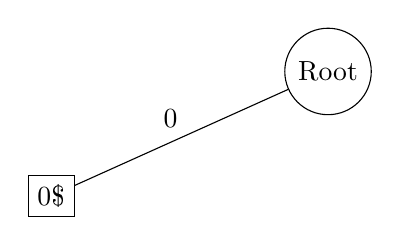
\begin{tikzpicture}[
  level distance=45 pt,
  level 1/.style={sibling distance=200 pt},
  level 2/.style={sibling distance=100 pt},
  level 3/.style={sibling distance=60 pt}
]
  \node[circle,draw] {Root}
      child {node[draw] {0\$}
    }
    child[missing];
  \node at (-2,-0.6) {0};
\end{tikzpicture}\end{center}
By our equation we get that height is $\lceil k \rceil + 1$, which gives us that the height 1 is, by inspecting the diagram we can see that is correct and so we can move onto the next step.\\\\
\textbf{Inductive hypothesis:} We will assume that a integer $i$ exists such that $i > k$ and such that the height of a tree made by inserting 0,1,...,$2^i-1$ elements is $\lceil i \rceil$. \\\\
\textbf{Inductive step:} We will now observe what will happen when we insert $i+1$ elements into the trie. the set of numbers we are inserting is $\{ 0, 1, ..., 2^i-1, 2^i, ..., 2^{i+1}-2, 2^{i+1}-1\}$. We can split this into two subsets:
\begin{align*}  
    \begin{aligned}
       \{0,1,.. 2^i-1\} & \{2^i, ..., 2^{i+1}-2, 2^{i+1}-1\}
    \end{aligned}
\end{align*}
From our I.H, we know that the first subset will form a tree of size i+1 (including the \$).  Each of the values in the second subset, will be equal to one of the second last level of the tree just with two extra values added (either a 0\$ or a 1\$), thus we can accommodate all $2^i$ nodes by adding an extra level. This will result in a tree with size $i+1$. Thus we have proved the hypothesis as $i+1$ result in a tree with height $i+1$.

\end{adjustwidth} 



\end{document}